% !TEX program = xelatex
% ============================================================================
%  POSN Computer Qualification — Triangles
%  Topic: สามเหลี่ยม (Triangles)
% ============================================================================

\documentclass[11pt, aspectratio=169]{beamer}
% ============================================================================
%  POSN Computer Qualification — Shared Beamer Preamble
%  Used by all topic slide decks. Compile with XeLaTeX.
% ============================================================================

% ---------- Thai language & font ----------
\usepackage{iftex}
\usepackage{fontspec}

% XeTeX-specific: enable Thai line breaking
\ifXeTeX
  \XeTeXlinebreaklocale{th}
\fi
% Noto Sans Thai — body text (clean modern sans-serif, handles all Thai)
\setmainfont{Noto Sans Thai}[
  UprightFont = Noto Sans Thai Light,
  BoldFont    = Noto Sans Thai Medium,
  Scale       = 0.9
]
\setsansfont{Noto Sans Thai}[
  UprightFont = Noto Sans Thai Light,
  BoldFont    = Noto Sans Thai Medium,
  Scale       = 0.9
]

% Noto Sans Thai — clean modern sans-serif for structural elements
\newfontfamily\headingfont{Noto Sans Thai}[
  UprightFont = Noto Sans Thai Medium,
  BoldFont    = Noto Sans Thai Bold,
  Scale       = 0.9
]

% --- Heading font for structural elements ---
\setbeamerfont{title}{family=\headingfont, series=\bfseries, size=\huge}
\setbeamerfont{subtitle}{family=\headingfont, series=\mdseries}
\setbeamerfont{author}{family=\headingfont, series=\mdseries}

% --- Custom Title Page ---
\defbeamertemplate{title page}{custom}[1][]{%
  \centering
  \vspace*{2cm}
  % Title — in white
  {\usebeamerfont{title}\color{white}\inserttitle\par}
  \vspace{0.6cm}
  % Subtitle — in white
  {\usebeamerfont{subtitle}\color{white}\insertsubtitle\par}
  \vspace{2.5cm}
  % Author — blue filled rounded box, white text
  \begin{center}
    \begin{tcolorbox}[arc=3mm, colback=boxBlue, colframe=boxBlue!80,
                      width=0.42\textwidth, halign=center,
                      left=1.5em, right=1.5em, top=0.8em, bottom=0.8em,
                      boxrule=1.5pt, coltext=white]
      \usebeamerfont{author}\insertauthor
    \end{tcolorbox}
  \end{center}
}
\setbeamertemplate{title page}[custom]
\setbeamerfont{frametitle}{family=\headingfont, series=\bfseries}
\setbeamerfont{section in toc}{family=\headingfont}
\setbeamerfont{page number in head/foot}{family=\headingfont}
\setbeamerfont{section title}{family=\headingfont, series=\bfseries}
\setbeamerfont{subsection title}{family=\headingfont}

% Monospace font (for code/verbatim)
\setmonofont{Latin Modern Mono}[Scale=0.9]

% ---------- Math ----------
\usepackage{amsmath, amssymb}

% ---------- Graphics ----------
\usepackage{graphicx}
\usepackage{tikz}

% ---------- String parsing (for section headers) ----------
\usepackage{xstring}

% ---------- Colored boxes ----------
\usepackage[skins, breakable, xparse]{tcolorbox}
% Note: we do NOT load the 'most' option — it predefines example/solution environments
% that would conflict with our custom boxes.

% --- Color definitions ---
\definecolor{boxBlue}{RGB}{41, 128, 185}
\definecolor{boxGreen}{RGB}{39, 174, 96}
\definecolor{boxOrange}{RGB}{230, 126, 34}
\definecolor{boxPurple}{RGB}{142, 68, 173}
\definecolor{boxBlueBg}{RGB}{235, 245, 255}
\definecolor{boxGreenBg}{RGB}{235, 255, 240}
\definecolor{boxOrangeBg}{RGB}{255, 245, 235}
\definecolor{boxPurpleBg}{RGB}{248, 240, 255}

% --- Explanation box (blue) — for definitions, concepts, notes ---
\newtcolorbox{explanation}[1][]{
  enhanced,
  breakable,
  arc         = 2mm,
  colback     = boxBlueBg,
  colframe    = boxBlue!50,
  title       = #1,
  fonttitle   = \bfseries\color{white},
  coltitle    = white,
  colbacktitle= boxBlue,
  attach boxed title to top left = {yshift=-2mm, xshift=2mm},
  boxed title style = {arc=2mm, size=small},
  before skip = 8pt,
  after skip  = 8pt
}

% --- Example box (green) — for worked examples ---
\newtcolorbox{exambox}[1][]{
  enhanced,
  breakable,
  arc         = 2mm,
  colback     = boxGreenBg,
  colframe    = boxGreen!50,
  title       = #1,
  fonttitle   = \bfseries\color{white},
  coltitle    = white,
  colbacktitle= boxGreen,
  attach boxed title to top left = {yshift=-2mm, xshift=2mm},
  boxed title style = {arc=2mm, size=small},
  before skip = 8pt,
  after skip  = 8pt
}

% --- Solution box (orange) — for solutions and answers ---
\newtcolorbox{solbox}[1][]{
  enhanced,
  breakable,
  arc         = 2mm,
  colback     = boxOrangeBg,
  colframe    = boxOrange!50,
  title       = #1,
  fonttitle   = \bfseries\color{white},
  coltitle    = white,
  colbacktitle= boxOrange,
  attach boxed title to top left = {yshift=-2mm, xshift=2mm},
  boxed title style = {arc=2mm, size=small},
  before skip = 8pt,
  after skip  = 8pt
}

% --- Intuition box (purple) — for plain-language explanations, analogies ---
\newtcolorbox{intuition}[1][]{
  enhanced,
  breakable,
  arc         = 2mm,
  colback     = boxPurpleBg,
  colframe    = boxPurple!50,
  title       = #1,
  fonttitle   = \bfseries\color{white},
  coltitle    = white,
  colbacktitle= boxPurple,
  attach boxed title to top left = {yshift=-2mm, xshift=2mm},
  boxed title style = {arc=2mm, size=small},
  before skip = 8pt,
  after skip  = 8pt
}

% ---------- Beamer theme ----------
\usetheme{Madrid}
\usecolortheme{default}

% --- Custom beamer colors (blue accent matching explanation boxes) ---
\setbeamercolor{structure}{fg=boxBlue}
\setbeamercolor{palette primary}{fg=white, bg=boxBlue}
\setbeamercolor{palette secondary}{fg=white, bg=boxBlue!80}
\setbeamercolor{palette tertiary}{fg=white, bg=boxBlue!60}
\setbeamercolor{block title}{fg=white, bg=boxBlue}
\setbeamercolor{block body}{fg=black, bg=boxBlueBg}

% Remove navigation symbols for clean look
\setbeamertemplate{navigation symbols}{}

% Note: Frame title prefix removed — \addtobeamertemplate conflicts with beamer internals

% --- Outline (Table of Contents) styling ---
\setbeamerfont{section in toc}{family=\headingfont, series=\mdseries}
\setbeamerfont{subsection in toc}{family=\headingfont, series=\mdseries}
\setbeamertemplate{section in toc}{%
  \leavevmode\leftskip=1.5em
  \textcolor{boxBlue}{\textbf{\large\inserttocsectionnumber.}}%
  \quad\inserttocsection\par
  \vspace{0.2em}
}
\setbeamertemplate{subsection in toc}{%
  \leavevmode\leftskip=4em
  \textcolor{boxBlue!60}{\small$\bullet$}%
  \quad\inserttocsubsection\par
  \vspace{0.1em}
}

% Section header slides — Thai in white, English in smaller light blue below
\AtBeginSection{
  \begin{frame}[plain]{}
    \vspace*{2cm}
    \begin{beamercolorbox}[sep=12pt, center, rounded=true, shadow=true]{palette primary}
      \IfSubStr{\secname}{(}{%
        \StrBefore{\secname}{(}[\sectionthai]%
        \StrBetween[1,1]{\secname}{(}{)}[\sectioneng]%
        \begin{tabular}{@{}c@{}}
          {\usebeamerfont{title}\sectionthai} \\[0.2em]
          {\usebeamerfont{subtitle}\color{boxBlue!60}\sectioneng}
        \end{tabular}%
      }{%
        {\usebeamerfont{title}\secname\par}%
      }
    \end{beamercolorbox}
    \vfill
  \end{frame}
}

% Subsection header slides — smaller, centered
\AtBeginSubsection{
  \begin{frame}[plain]{}
    \vfill
    \centering
    {\usebeamerfont{section title}\insertsubsectionhead\par}
    \vfill
  \end{frame}
}

% Minimal footer: page number only, right-aligned
\setbeamertemplate{footline}{
  \hfill\usebeamerfont{page number in head/foot}\insertframenumber{} / \inserttotalframenumber\hspace*{1em}\vspace*{0.5ex}
}

% ---------- Spacing & readability ----------
\linespread{1.2}

% ---------- Useful commands ----------

% Highlight important text in blue
\newcommand{\highlight}[1]{\textcolor{boxBlue}{\textbf{#1}}}

% Math set notation helpers
\newcommand{\R}{\mathbb{R}}
\newcommand{\N}{\mathbb{N}}
\newcommand{\Z}{\mathbb{Z}}
\newcommand{\Q}{\mathbb{Q}}

% ============================================================================
%  End of preamble
% ============================================================================


\title[สามเหลี่ยม]{\textcolor{white}{สามเหลี่ยม} \textcolor{boxBlue!60}{(Triangles)}}
\subtitle{ชนิด • ความเท่ากันทุกประการ • ความคล้าย • ทฤษฎีบทพีทาโกรัส }
\author[None W. (Yuan)]{None W. (Yuan)}
\date{}

\begin{document}

\begin{frame}[plain]\titlepage\end{frame}
\begin{frame}{สารบัญ (Outline)}\tableofcontents\end{frame}

\begin{frame}{ก่อนเรียน (Prerequisites)}
  \begin{explanation}[สิ่งที่ควรรู้ก่อนเรียน]
    \begin{itemize}
      \item \textbf{มุม} — ชนิดของมุม, มุมประกอบ, มุมตรงข้าม, มุมในเส้นขนาน
      \item \textbf{สมการ} — การแก้สมการเชิงเส้น, การแยกตัวประกอบ
      \item \textbf{เลขยกกำลัง} — $a^2$, $\sqrt{a}$
    \end{itemize}
  \end{explanation}
  \begin{intuition}[สามเหลี่ยมคืออะไร?]
    รูปหลายเหลี่ยมที่มี 3 ด้าน 3 มุม — เป็นรูปพื้นฐานที่สุดในเรขาคณิต
    สามเหลี่ยมทุกชนิดมีผลรวมมุมภายใน $= 180^\circ$
  \end{intuition}
\end{frame}

% ===========================================================================
%  SECTION 1: ชนิดของรูปสามเหลี่ยม
% ===========================================================================
\section{ชนิดของรูปสามเหลี่ยม (Types of Triangles)}

\begin{frame}{จำแนกตามด้าน}
  \begin{columns}[T]
    \column{0.33\textwidth}
      \centering
      \textbf{ด้านเท่า (Equilateral)} \par 3 ด้านเท่ากัน, 3 มุม $= 60^\circ$

      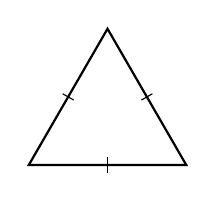
\begin{tikzpicture}[scale=1]
        \draw[thick] (0,0) -- (2,0) -- (1,1.73) -- cycle;
        % base: one tick at midpoint, perpendicular to horizontal
        \draw (1,0.1) -- (1,-0.1);
        % left side (0,0)-(1,1.73): midpoint (0.5,0.865), dir 60°, perp 150°
        \draw (0.43,0.905) -- (0.57,0.825);
        % right side (2,0)-(1,1.73): midpoint (1.5,0.865), dir 120°, perp 30°
        \draw (1.43,0.825) -- (1.57,0.905);
      \end{tikzpicture}

    \column{0.33\textwidth}
      \centering
      \textbf{หน้าจั่ว (Isosceles)} \par 2 ด้านเท่ากัน, มุมฐานเท่ากัน

      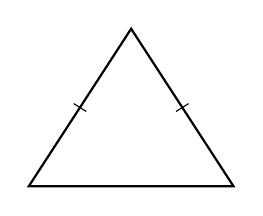
\begin{tikzpicture}[scale=1]
        \draw[thick] (0,0) -- (2.6,0) -- (1.3,2) -- cycle;
        % left equal side (0,0)-(1.3,2): midpoint (0.65,1), dir 57°, perp 147°
        \draw (0.57,1.05) -- (0.73,0.95);
        % right equal side (1.3,2)-(2.6,0): midpoint (1.95,1), dir 123°, perp 33°
        \draw (1.87,0.95) -- (2.03,1.05);
      \end{tikzpicture}

    \column{0.33\textwidth}
      \centering
      \textbf{ด้านไม่เท่า (Scalene)} \par 3 ด้านไม่เท่ากันเลย

      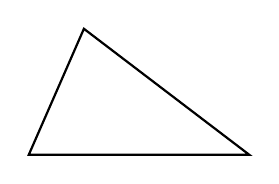
\begin{tikzpicture}[scale=1]
        \draw[thick] (0,0) -- (2.8,0) -- (0.7,1.6) -- cycle;
      \end{tikzpicture}
  \end{columns}
\end{frame}

\begin{frame}{จำแนกตามมุม}
  \begin{columns}[T]
    \column{0.33\textwidth}
      \centering
      \textbf{มุมแหลม (Acute)} \par ทุกมุม $< 90^\circ$

      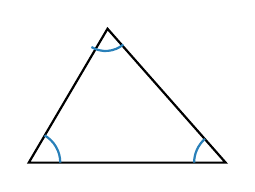
\begin{tikzpicture}[scale=1]
        \draw[thick] (0,0) -- (2.5,0) -- (1,1.7) -- cycle;
        \draw[boxBlue, thick] (0.4,0) arc (0:60:0.4);
        \draw[boxBlue, thick] (2.1,0) arc (180:131:0.4);
        \draw[boxBlue, thick] (1.2,1.5) arc (-50:-121:0.35);
      \end{tikzpicture}

    \column{0.33\textwidth}
      \centering
      \textbf{มุมฉาก (Right)} \par 1 มุม $= 90^\circ$

      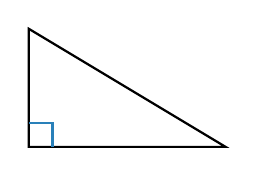
\begin{tikzpicture}[scale=1]
        \draw[thick] (0,0) -- (2.5,0) -- (0,1.5) -- cycle;
        \draw[boxBlue, thick] (0.3,0) -- (0.3,0.3) -- (0,0.3);
      \end{tikzpicture}

    \column{0.33\textwidth}
      \centering
      \textbf{มุมป้าน (Obtuse)} \par 1 มุม $> 90^\circ$

      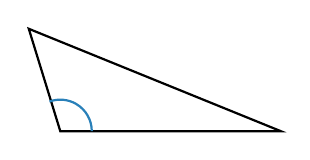
\begin{tikzpicture}[scale=1]
        \draw[thick] (0,0) -- (2.8,0) -- (-0.4,1.3) -- cycle;
        \draw[boxBlue, thick] (0.4,0) arc (0:110:0.4);
      \end{tikzpicture}
  \end{columns}
\end{frame}

% ===========================================================================
%  SECTION 2: ความเท่ากันทุกประการ (Congruence)
% ===========================================================================
\section{ความเท่ากันทุกประการ (Congruence)}

\begin{frame}{สามเหลี่ยมเท่ากันทุกประการ}
  \begin{explanation}[นิยาม]
    สามเหลี่ยมสองรูป \highlight{เท่ากันทุกประการ} ($\cong$) ก็ต่อเมื่อ
    มีขนาดและรูปร่างเหมือนกัน — ด้านเท่ากันและมุมเท่ากัน
  \end{explanation}

  \begin{columns}[T]
    \column{0.25\textwidth}
      \centering \small
      \textbf{SSS} \par 3 ด้านเท่ากัน

      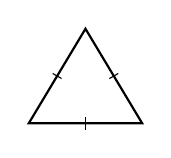
\begin{tikzpicture}[scale=0.8]
        \draw[thick] (0,0) -- (1.8,0) -- (0.9,1.5) -- cycle;
        % base tick: midpoint (0.9,0), vertical
        \draw (0.9,0.1) -- (0.9,-0.1);
        % left side tick: midpoint (0.45,0.75), dir 59°, perp 149°
        \draw (0.38,0.79) -- (0.52,0.71);
        % right side tick: midpoint (1.35,0.75), dir 121°, perp 31°
        \draw (1.28,0.71) -- (1.42,0.79);
      \end{tikzpicture}

    \column{0.25\textwidth}
      \centering \small
      \textbf{SAS} \par 2 ด้าน + มุมระหว่าง

      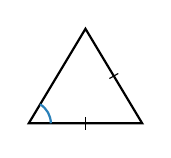
\begin{tikzpicture}[scale=0.8]
        \draw[thick] (0,0) -- (1.8,0) -- (0.9,1.5) -- cycle;
        % base tick: midpoint (0.9,0)
        \draw (0.9,0.1) -- (0.9,-0.1);
        % right side tick: midpoint (1.35,0.75)
        \draw (1.28,0.71) -- (1.42,0.79);
        % angle arc at bottom-left
        \draw[boxBlue, thick] (0.35,0) arc (0:59:0.35);
      \end{tikzpicture}

    \column{0.25\textwidth}
      \centering \small
      \textbf{ASA} \par 2 มุม + ด้านระหว่าง

      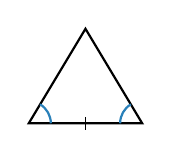
\begin{tikzpicture}[scale=0.8]
        \draw[thick] (0,0) -- (1.8,0) -- (0.9,1.5) -- cycle;
        % base tick: midpoint (0.9,0)
        \draw (0.9,0.1) -- (0.9,-0.1);
        % two angle arcs
        \draw[boxBlue, thick] (0.35,0) arc (0:59:0.35);
        \draw[boxBlue, thick] (1.45,0) arc (180:121:0.35);
      \end{tikzpicture}

    \column{0.25\textwidth}
      \centering \small
      \textbf{RHS} \par มุมฉาก+ด้านตรงข้าม+ด้านประกอบ

      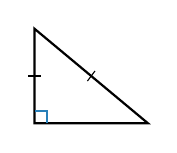
\begin{tikzpicture}[scale=0.8]
        \draw[thick] (0,0) -- (1.8,0) -- (0,1.5) -- cycle;
        % right angle marker
        \draw[boxBlue, thick] (0.2,0) -- (0.2,0.2) -- (0,0.2);
        % hypotenuse tick: (0,1.5)-(1.8,0), midpoint (0.9,0.75), dir -40°, perp 50°
        \draw (0.84,0.67) -- (0.96,0.83);
        % vertical leg tick: (0,0)-(0,1.5), midpoint (0,0.75), horizontal
        \draw (-0.1,0.75) -- (0.1,0.75);
      \end{tikzpicture}
  \end{columns}
\end{frame}

% ===========================================================================
%  SECTION 3: ความคล้าย (Similarity)
% ===========================================================================
\section{ความคล้าย (Similarity)}

\begin{frame}{สามเหลี่ยมคล้ายกัน}
  \begin{explanation}[นิยาม]
    สามเหลี่ยมสองรูป \highlight{คล้ายกัน} ($\sim$) ก็ต่อเมื่อ
    มีรูปร่างเหมือนกัน แต่อาจมีขนาดต่างกัน
  \end{explanation}

  \begin{center}
    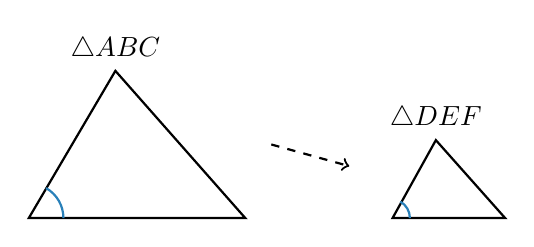
\begin{tikzpicture}[scale=1.1]
      % Big triangle
      \draw[thick] (0,0) -- (2.5,0) -- (1,1.7) -- cycle;
      \node at (1,1.95) {$\triangle ABC$};
      \draw[boxBlue, thick] (0.4,0) arc (0:60:0.4);

      % Arrow
      \draw[->, thick, dashed] (2.8,0.85) -- (3.7,0.6);

      % Small triangle (scaled manually)
      \draw[thick] (4.2,0) -- (5.5,0) -- (4.7,0.9) -- cycle;
      \node at (4.7,1.15) {$\triangle DEF$};
      \draw[boxBlue, thick] (4.4,0) arc (0:60:0.22);
    \end{tikzpicture}
  \end{center}

  \begin{itemize}
    \item มุมทั้ง 3 เท่ากัน \quad $\bullet$ \quad อัตราส่วนด้านคู่ที่สมนัยกันเท่ากัน
  \end{itemize}
\end{frame}

\begin{frame}{เงื่อนไขความคล้าย}
  \begin{columns}[T]
    \column{0.33\textwidth}
      \centering \small
      \textbf{AAA} \par 3 มุมเท่ากัน = คล้ายกัน

      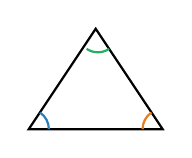
\begin{tikzpicture}[scale=0.85]
        \draw[thick] (0,0) -- (2,0) -- (1,1.5) -- cycle;
        \draw[boxBlue, thick] (0.3,0) arc (0:56:0.3);
        \draw[boxOrange, thick] (1.7,0) arc (180:124:0.3);
        \draw[boxGreen, thick] (1.2,1.2) arc (-56:-124:0.3);
      \end{tikzpicture}

    \column{0.33\textwidth}
      \centering \small
      \textbf{SAS (ratio)} \par 2 ด้านได้สัดส่วน + มุมระหว่างเท่ากัน

      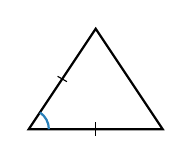
\begin{tikzpicture}[scale=0.85]
        \draw[thick] (0,0) -- (2,0) -- (1,1.5) -- cycle;
        \draw[boxBlue, thick] (0.3,0) arc (0:56:0.3);
        % base tick: midpoint (1,0)
        \draw (1,0.1) -- (1,-0.1);
        % left side tick: midpoint (0.5,0.75)
        \draw (0.43,0.79) -- (0.57,0.71);
      \end{tikzpicture}

    \column{0.33\textwidth}
      \centering \small
      \textbf{SSS (ratio)} \par อัตราส่วน 3 ด้านเท่ากัน

      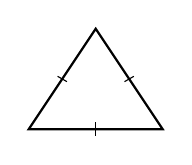
\begin{tikzpicture}[scale=0.85]
        \draw[thick] (0,0) -- (2,0) -- (1,1.5) -- cycle;
        % base tick: midpoint (1,0)
        \draw (1,0.1) -- (1,-0.1);
        % left side tick: midpoint (0.5,0.75)
        \draw (0.43,0.79) -- (0.57,0.71);
        % right side tick: midpoint (1.5,0.75)
        \draw (1.43,0.71) -- (1.57,0.79);
      \end{tikzpicture}
  \end{columns}
\end{frame}

\begin{frame}{ตัวอย่าง: ความคล้าย}
  \begin{exambox}[โจทย์]
    $\triangle ABC \sim \triangle DEF$, $AB = 6$, $BC = 8$, $DE = 3$ \quad จงหา $EF$
  \end{exambox}

  \begin{solbox}[วิธีทำ]
    อัตราส่วน: $\dfrac{AB}{DE} = \dfrac{6}{3} = 2$

    ดังนั้น $\dfrac{BC}{EF} = 2 \;\Rightarrow\; \dfrac{8}{EF} = 2 \;\Rightarrow\; EF = 4$
  \end{solbox}

  \begin{intuition}[การนำไปใช้]
    ความคล้ายใช้ในการวัดความสูงของสิ่งที่ไม่สามารถวัดได้โดยตรง เช่น ความสูงของตึกโดยใช้เงา
  \end{intuition}
\end{frame}

% ===========================================================================
%  SECTION 4: ทฤษฎีบทพีทาโกรัส
% ===========================================================================
\section{ทฤษฎีบทพีทาโกรัส (Pythagorean Theorem)}

\begin{frame}{ทฤษฎีบทพีทาโกรัส}
  \begin{explanation}[ทฤษฎีบท]
    ในรูปสามเหลี่ยมมุมฉาก \highlight{$c^2 = a^2 + b^2$}
  \end{explanation}

  \begin{center}
    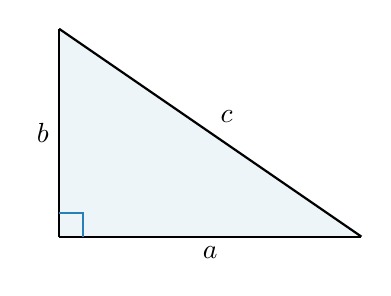
\begin{tikzpicture}[scale=1.2]
      \fill[boxBlue!8] (0,0) -- (3.2,0) -- (0,2.2) -- cycle;
      \draw[thick] (0,0) -- (3.2,0) node[midway, below] {$a$};
      \draw[thick] (0,0) -- (0,2.2) node[midway, left] {$b$};
      \draw[thick] (0,2.2) -- (3.2,0) node[midway, above right] {$c$};
      \draw[boxBlue, thick] (0.25,0) -- (0.25,0.25) -- (0,0.25);
    \end{tikzpicture}
  \end{center}

  \begin{exambox}[ตัวอย่าง]
    $a = 3$, $b = 4$ \quad $\rightarrow$ \quad $c = \sqrt{3^2 + 4^2} = \sqrt{25} = 5$
  \end{exambox}
\end{frame}

\begin{frame}{บทกลับของทฤษฎีบทพีทาโกรัส}
  \begin{explanation}[บทกลับ]
    ถ้า $c^2 = a^2 + b^2$ แล้วสามเหลี่ยมนั้นเป็นสามเหลี่ยมมุมฉาก ($c$ คือด้านยาวสุด)
  \end{explanation}

  \begin{exambox}[ตัวอย่าง: ด้าน 5 12 13]
    $13^2 = 169$, \quad $5^2 + 12^2 = 25 + 144 = 169$

    $13^2 = 5^2 + 12^2$ $\rightarrow$ เป็นสามเหลี่ยมมุมฉาก!
  \end{exambox}

  \begin{intuition}[เลขพีทาโกรัส]
    ชุดที่พบบ่อย: $(3,4,5)$, $(5,12,13)$, $(6,8,10)$, $(8,15,17)$, $(9,12,15)$
  \end{intuition}
\end{frame}

% ===========================================================================
%  SECTION 5: สามเหลี่ยมมุมฉากพิเศษ
% ===========================================================================
\section{สามเหลี่ยมมุมฉากพิเศษ (Special Right Triangles)}

\begin{frame}{สามเหลี่ยม $45^\circ$-$45^\circ$-$90^\circ$}
  \begin{columns}[T]
    \column{0.5\textwidth}
      \centering
      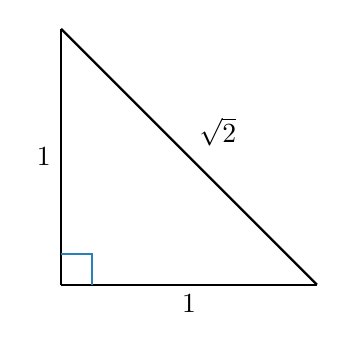
\begin{tikzpicture}[scale=1.3]
        \draw[thick] (0,0) -- (2.5,0) node[midway, below] {$1$};
        \draw[thick] (0,0) -- (0,2.5) node[midway, left] {$1$};
        \draw[thick] (0,2.5) -- (2.5,0) node[midway, above right] {$\sqrt{2}$};
        \draw[boxBlue, thick] (0.3,0) -- (0.3,0.3) -- (0,0.3);
      \end{tikzpicture}

    \column{0.5\textwidth}
      \begin{explanation}[อัตราส่วน]
        ด้าน : ด้าน : ด้านตรงข้ามมุมฉาก
        \[ 1 : 1 : \sqrt{2} \]
        คูณด้วย $k$: \quad $k : k : k\sqrt{2}$
      \end{explanation}
  \end{columns}
\end{frame}

\begin{frame}{สามเหลี่ยม $30^\circ$-$60^\circ$-$90^\circ$}
  \begin{columns}[T]
    \column{0.5\textwidth}
      \centering
      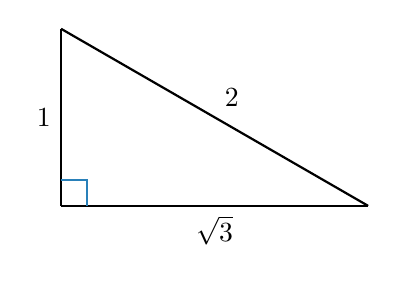
\begin{tikzpicture}[scale=1.3]
        \draw[thick] (0,0) -- (3,0) node[midway, below] {$\sqrt{3}$};
        \draw[thick] (0,0) -- (0,1.73) node[midway, left] {$1$};
        \draw[thick] (0,1.73) -- (3,0) node[midway, above right] {$2$};
        \draw[boxBlue, thick] (0.25,0) -- (0.25,0.25) -- (0,0.25);
      \end{tikzpicture}

    \column{0.5\textwidth}
      \begin{explanation}[อัตราส่วน]
        $30^\circ$ ตรงข้าม $1$
        \par $60^\circ$ ตรงข้าม $\sqrt{3}$
        \par $90^\circ$ ตรงข้าม $2$
        \medskip
        คูณด้วย $k$: \quad $k : k\sqrt{3} : 2k$
      \end{explanation}
  \end{columns}
\end{frame}

% ===========================================================================
%  SUMMARY
% ===========================================================================
\section{สรุป}

\begin{frame}{สรุปเนื้อหา}
  \begin{explanation}[สิ่งที่ได้เรียนรู้]
    \begin{enumerate}
      \item \textbf{ชนิด}: ด้านเท่า/หน้าจั่ว/ด้านไม่เท่า, แหลม/ฉาก/ป้าน
      \item \textbf{ความเท่ากันทุกประการ} ($\cong$): SSS, SAS, ASA, RHS
      \item \textbf{ความคล้าย} ($\sim$): AAA, SAS (ratio), SSS (ratio)
      \item \textbf{พีทาโกรัส}: $c^2 = a^2 + b^2$ — บทกลับใช้ทดสอบสามเหลี่ยมมุมฉาก
      \item \textbf{สามเหลี่ยมพิเศษ}: $45^\circ$-$45^\circ$-$90^\circ$ ($1:1:\sqrt{2}$), $30^\circ$-$60^\circ$-$90^\circ$ ($1:\sqrt{3}:2$)
    \end{enumerate}
  \end{explanation}
  \begin{center}
    \large เอกสารนี้เป็นส่วนหนึ่งของเนื้อหาเตรียมสอบ \textbf{สอวน. คอมพิวเตอร์}
  \end{center}
\end{frame}

\end{document}
